 \documentclass[compress,xcolor=table]{beamer}
\usepackage[french]{babel}
\selectlanguage{french}
\usepackage[utf8]{inputenc}
\usepackage[T1]{fontenc}

\usepackage{tikz}
\usepackage{pdfpages}
\usepackage{dirtree}

\usetheme{edts}

% remove some frames for navigation
\makeatletter
\let\beamer@writeslidentry@miniframeson=\beamer@writeslidentry
\def\beamer@writeslidentry@miniframesoff{%
  \expandafter\beamer@ifempty\expandafter{\beamer@framestartpage}{}% does not happen normally
  {%else
    % removed \addtocontents commands
    \clearpage\beamer@notesactions%
  }
}
\newcommand*{\miniframeson}{\let\beamer@writeslidentry=\beamer@writeslidentry@miniframeson}
\newcommand*{\miniframesoff}{\let\beamer@writeslidentry=\beamer@writeslidentry@miniframesoff}
\makeatother
% end remove frames from navigation


\title{Détection de rupture dans une vidéo}
\subtitle{Soutenance de projet d'EDTS}
\date{\today}
\author{Ya \textsc{Huang} \and Rémi \textsc{Mussard} \and Thomas \textsc{Robert}}
\institute{Institut National des Sciences Appliquées de Rouen}

\setbeameroption{show notes}

\DeclareMathOperator*{\argmax}{arg\,max}
\DeclareMathOperator*{\randperm}{randperm}
\begin{document}

\begin{frame}[plain]
	\titlepage
    \setcounter{framenumber}{0}
\end{frame}

\begin{frame}{Sommaire}
\begin{minipage}{\textwidth}
   \linespread{1.35}
	\tableofcontents[hideallsubsections]
\end{minipage}
\end{frame}

\section{Extraction de caractéristiques}
\subsection{}
\chapter{Extraction de caractéristiques}

\section{Texture}

Dans le cadre de la détection de rupture, une autre caractéristique intéressante à exploiter est la texture des images. Différentes approches sont possibles pour représenter mathématiquement une texture. Pour ce projet, nous nous sommes intéressés à une approche statistique, avec la matrice de cooccurrence.

\subsection{Définition d'une texture}

En traitement d'image, on défini une texture comme étant \textit{une région spatiale d'une image présentant une organisation spatiale homogène des niveaux de luminance}. Une texture consiste en une reproduction de motifs de base dans l'espace et dans plusieurs directions. Ces motifs (ou primitives) sont organisés les uns par rapport aux autres de manière aléatoire.\\

D'après cette définition, on peut considérer une texture comme une structure à deux dimensions :

\begin{itemize}
    \item La première dimension représente les primitives formant la texture ;
    \item La seconde dimension représente l'organisation spatiale de ces primitives entre elles.
\end{itemize}

On recense deux types de texture, les macrotextures et les microtextures.

\begin{itemize}
    \item Une \textbf{macrotexture} est une texture structurée, pour laquelle on peut extraire facilement un motif de base et les lois d'assemblage des primitives entre elles. Par exemple, la texture d'un mur de briques est une macrotexture ;
    \item Une \textbf{microtexture} est une texture aléatoire, avec un aspect désorganisé, mais qui donne une impression visuelle relativement homogène. On peut prendre l'exemple d'une vue aérienne sur un champs.
\end{itemize}

Cependant, il est parfois difficile de classer une texture dans une catégorie ou l'autre. En fonction de la résolution de l'image ou du zoom effectué sur celle-ci, on va préférer classer la texture dans l'une ou l'autre des catégories. On peut prendre l'exemple du sable, dans le cas où aucun zoom n'est effectué (\ref{noZoom}), il est tentant de classer cette texture en tant que macrotexture, alors que dans le cas où un zoom est effectué (\ref{Zoom}), il est plus probable de classer cette texture en tant que microtexture.

\begin{figure}
   \begin{minipage}[c]{.46\linewidth}
	  \centering
      
\includegraphics[scale=0.16]{images/sableNoZoom.jpg}
      \caption{\label{noZoom} Sable non zoomé}
   \end{minipage} \hfill
   \begin{minipage}[c]{.46\linewidth}
      \centering
      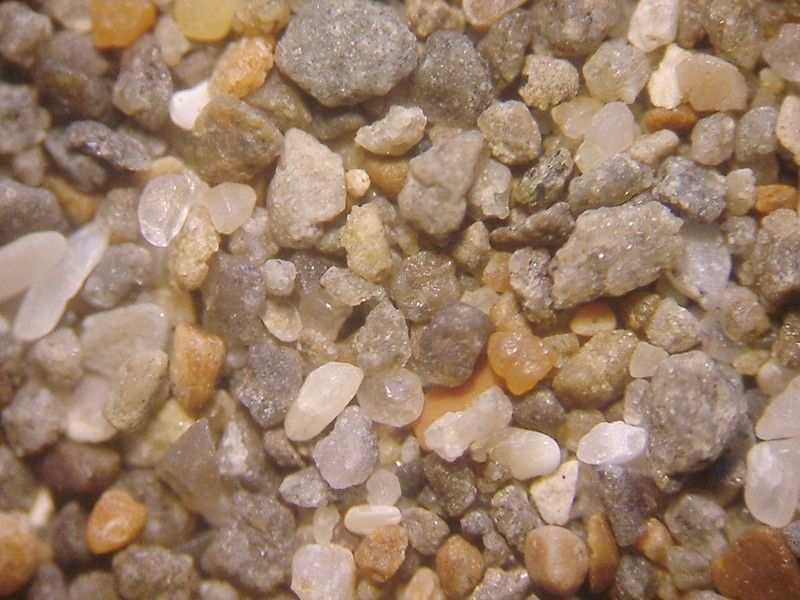
\includegraphics[scale=0.2]{images/sableZoom.jpg}
      \caption{\label{Zoom} Sable zoomé}
   \end{minipage}
\end{figure}

Il est important de retenir qu'une texture est une région d'une image pour laquelle il est possible de définir une fenêtre telle que pour toute translation de cette dernière, on retrouve le même motif. Une texture peut être décrite spatialement ou statistiquement. C'est cette dernière solution que nous tâcherons d'expliquer dans le cadre de ce projet, avec la matrice de cooccurrence.

\subsection{Matrice de cooccurrence}

En analyse de texture, cette méthode statistique donne des résultats relativement bons. Cette méthode consiste à compter le nombre de paires similaires de pixels ayant une distance $d$ entre eux. Cette méthode se base sur le niveau de gris des pixels, allant de 1 à 8. On prend également en compte la direction de la paire de pixels avec un angle $\theta$. Cette angle varie généralement entre $0$ et $180 degres$. Les pixels d'une paire sont généralement séparés par une distance $d=1$ pixel.\\

Si on prend les paramètres suivants, $d=1, \theta = 0$, on obtient une paire de pixel comme suit :

\[
 \left \{
 \begin{array}{c @{=} c}
     pix_1 & (x_1, y_1) \\
     pix_2 & (x_2, y_2) \\
 \end{array}
 \right.
\]

avec $x_2 = x_1 + 1$ et $y_2 = y_1$.\\

Le pixel $pix_2$ est donc le voisin de droite du pixel $pix_1$. La matrice de cooccurrence est une matrice carrée $n\times n$, avec $n$ le niveau de gris (égale à 8 dans notre cas). Elle va recenser le nombre de pixels ayant un niveau de gris $n2$, situé à la droite d'un pixel dont le niveau de gris est $n1$. Les lignes de la matrice de cooccurrence représentent les pixels de référence et les colonnes, les pixels situés à droite du pixel de référence. Soit l'image $I$ dont les pixels ont les niveaux de gris suivants :

\[
 I = \begin{pmatrix}
     1 & 8 & 1 & 8 \\
     2 & 1 & 1 & 8 \\
     5 & 4 & 3 & 7 \\     
 \end{pmatrix}
\]

La matrice de cooccurrence de $I$ sera donc :

\[
 C = \begin{pmatrix}
     1 & 0 & 0 & 0 & 0 & 0 & 0 & 3 \\
     1 & 0 & 0 & 0 & 0 & 0 & 0 & 0 \\
     0 & 0 & 0 & 0 & 0 & 0 & 1 & 0 \\
     0 & 0 & 1 & 0 & 0 & 0 & 0 & 0 \\
     0 & 0 & 0 & 1 & 0 & 0 & 0 & 0 \\
     0 & 0 & 0 & 0 & 0 & 0 & 0 & 0 \\
     0 & 0 & 0 & 0 & 0 & 0 & 0 & 0 \\
     1 & 0 & 0 & 0 & 0 & 0 & 0 & 0 \\   
 \end{pmatrix}
\]

La valeur $C(1, 8) = 3$ signifie qu'il y a trois fois un pixel de niveau de gris $8$ à la droite d'un pixel de niveau de gris $1$.

\subsection{Détection de rupture et matrice de cooccurrence}

Voyons à présent en quoi la matrice de cooccurrence permet de détecter des ruptures dans une vidéo. Dans une vidéo, deux images consécutives seront relativement proches l'une de l'autre, excepté en cas de rupture. La matrice de cooccurrence va permettre d'obtenir une description de la texture de l'image. Entre deux images d'une même scène, la texture ne devrait pas changer et on devrait avoir deux matrices de cooccurrence très proches. Il faut rappeler que la texture d'une image est basée sur la répétition de motifs, et donc, dans une scène, on devrait retrouver les mêmes motifs. Dans notre cas, dans une même scène, les niveaux de gris ne devraient pas énormément évoluer d'une image à l'autre.\\

La méthode des matrices de cooccurrence possède certains avantages, mais également quelques inconvénients.

\subsection{Avantages}

Les avantages de cette méthode sont les suivants :

\begin{itemize}
	\item Simple à mettre en oeuvre ;
	\item Relativement robuste aux changements d'intensité d'une couleur ;
	\item Relativement robuste aux transitions avec un effet de fondu.
\end{itemize}

\subsection{Inconvénients}

Les inconvénients de cette méthode sont les suivants :

\begin{itemize}
	\item Peu robuste aux changement d'angles de caméra ;
	\item Peu robuste à l'apparition de nouveaux objets sur une scène.
\end{itemize}


\section{Détection de rupture}
\subsection{}
\begin{frame}{Introduction}

\begin{exampleblock}{Données}
\begin{itemize}
\item Matrice de signal $X \in \mathbb{R}^{n \times p}$
\item $n$ observations dans le temps, 1 par image
\item $p$ caractéristiques extraites des images
\end{itemize}
\end{exampleblock}

\begin{block}{Objectif}
Déterminer les ruptures dans la vidéo au travers des caractéristiques extraites, dont la distribution est supposée stationnaire pour une séquence donnée.
\end{block}

\end{frame}

\begin{frame}{Prétraitement des caractéristiques}

{
\definecolor{tempGreen}{HTML}{96EAC0}
\setbeamercolor{block body example}{use=structure,fg=black,bg=tempGreen}
\begin{exampleblock}{Caractéristiques obtenues}
\centering
\includegraphics<1>[width=\textwidth]{images/signal}
\includegraphics<2>[width=.6\textwidth]{images/signal}
\end{exampleblock}
}

\begin{alertblock}<2>{Remarque}
	Peu de valeurs éloignées de 0 \\
	$\Rightarrow$ Prétraitement de la matrice de caractéristiques
\end{alertblock}
\end{frame}

\begin{frame}{Prétraitement des caractéristiques}{Résultat}

{
\definecolor{tempGreen}{HTML}{96EAC0}
\setbeamercolor{block body example}{use=structure,fg=black,bg=tempGreen}
\begin{exampleblock}{Caractéristiques après prétraitement ($\log (10^9 X + 1)$)}
\centering
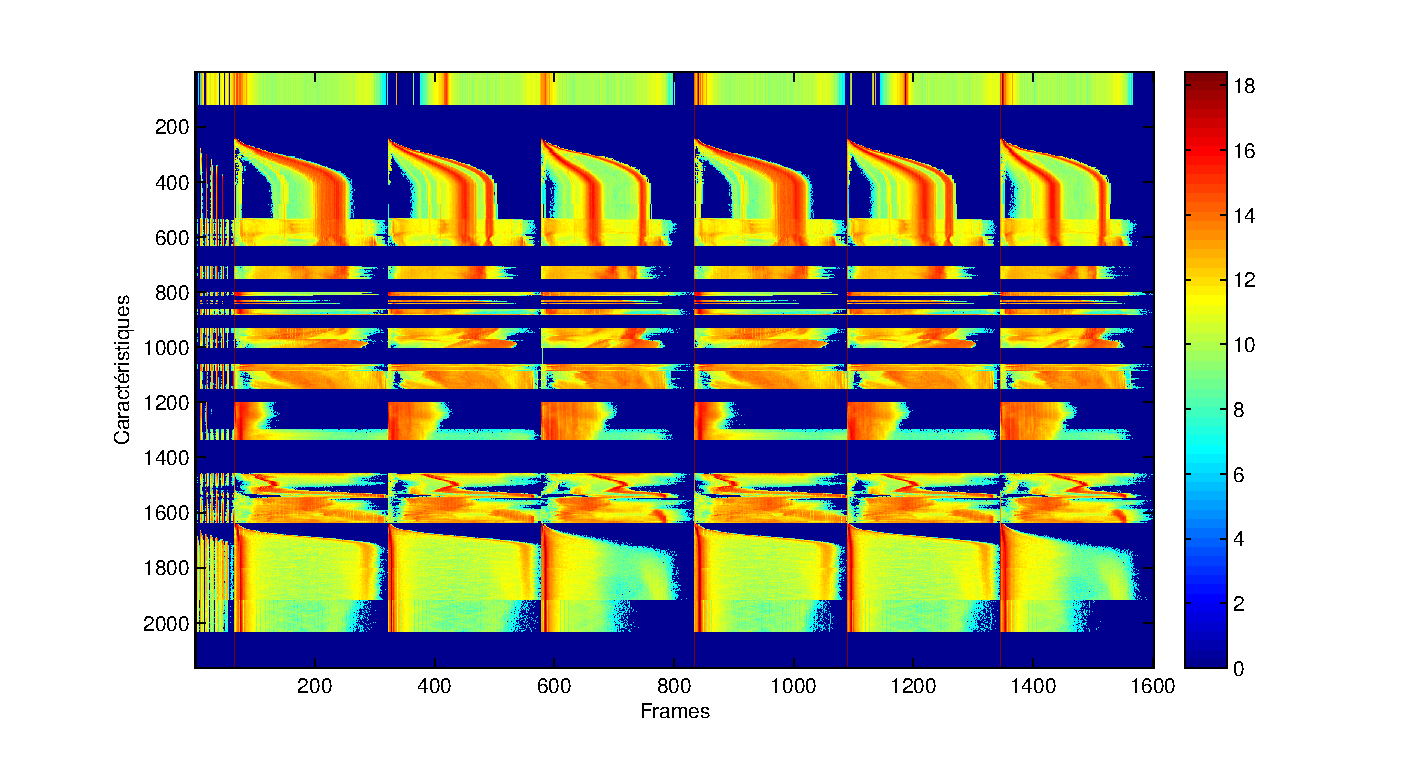
\includegraphics[width=\textwidth]{images/signalPreprocessed}
\end{exampleblock}
}

\end{frame}


\begin{frame}{Méthodes essayées}

\begin{alertblock}{Méthodes essayées}
\begin{itemize}
\item Méthode par dérivée filtrée utilisant la $p$-valeur\\
\textit{Source : \cite{Bertrand11} et \cite{Herault14}}
\item Méthode de détection de changement de noyau\\
\textit{Source : \cite{Desobry05}}
\end{itemize}
\end{alertblock}

\end{frame}


\begin{frame}{Dérivée filtrée}{Principe}

\begin{center}
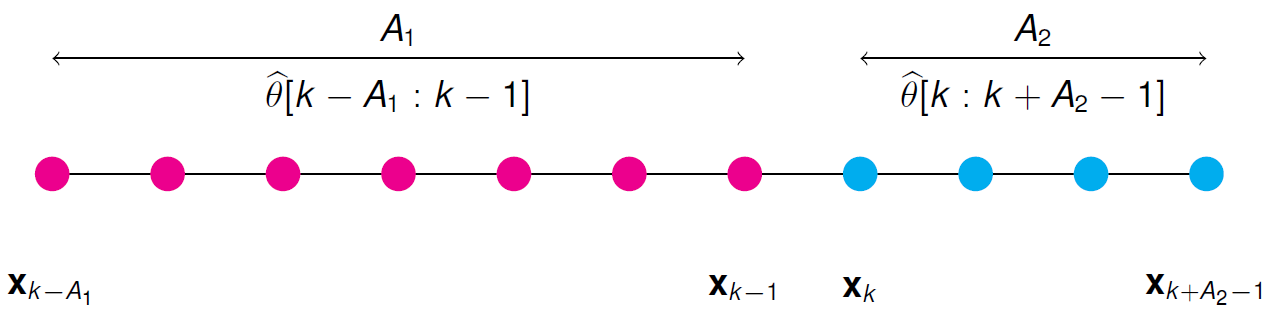
\includegraphics[width=0.8\textwidth]{images/deriveeFiltree}
\end{center}

\begin{block}{Principe}
\begin{itemize}
\item Parcours du signal avec deux fenêtre de taille $A_1$ et $A_2$
\item Distance $D(k)$ entre indicateurs $\hat{\theta}$ sur chaque fenêtre
\item Zones de rupture $\mathcal{K}_i = \{k \text{ successifs t.q. } |D(k)| > C\}$
\item Rupture en $k_{r_i} = \displaystyle \argmax_{k \in \mathcal{K}_i} |D(k)| \hspace{1em}\forall i$
\end{itemize}
\end{block}


\end{frame}

\begin{frame}{Dérivée filtrée}{Détermination de $C$}

\begin{block}{Principe probabiliste basée sur la $p$-valeur}
\vspace{-.7em}
\begin{itemize}
\item Hypothèse $\mathcal{H}_0$ : il n'y a pas de rupture
\item $M = \displaystyle \max_{k} |D(k)|$
\item On veut $C$ tel que $\mathbb{P}(M>C\mid	\mathcal{H}_0) < p$ avec $p$ fixé
\end{itemize}
\end{block}

\begin{exampleblock}{Méthode d'estimation de $C$}
\vspace{-.7em}
\begin{itemize}
\item Création de $\{X_{\mathcal{H}_0}\} = \{\randperm{(X)}\}$ données sous $\mathcal{H}_0$
\item Estimation de $\{M_{\mathcal{H}_0}\}$ sur ces données
\item Estimation de la distribution de $M$ sous $\mathcal{H}_0$
\item Estimation de $C$ tel que $\mathbb{P}(M>C\mid	\mathcal{H}_0) < p$
\end{itemize}
\end{exampleblock}

\end{frame}

\begin{frame}{Changement de noyau}{Principe}

\begin{block}{Principe}
\vspace{-.7em}
\begin{itemize}
\item Cas particulier de la dérivée filtrée
\item Indicateurs $\hat{\theta}$ étant les paramètres d'un \textit{one-class SVM} sur chaque fenêtre
\item Mesure de distance particulière entre les kernels
\end{itemize}
\end{block}

\end{frame}

\begin{frame}{Changement de noyau}{Distance}

\begin{columns}
\begin{column}{.47\textwidth}
\small
\begin{align}
  D &= \frac{\overset{\frown}{c_1 c_2}}{\overset{\frown}{c_1 p_1} + \overset{\frown}{c_2 p_2}} \notag \\
  \overset{\frown}{c_1 c_2} &= \arccos\left(\frac{
    	\langle w_1, w_2\rangle_\mathcal{H}
    	}{
    	\|w_1\|_\mathcal{H}\|w_2\|_\mathcal{H}
    	} \right) \notag \\
   &= \arccos\left(\frac{
  	\alpha_1^\top K_{12} \alpha_2
  	}{
  	\sqrt{\alpha_1^\top K_{11} \alpha_1} \sqrt{\alpha_2^\top K_{22} \alpha_2}
  	} \right) \notag \\
  \overset{\frown}{c_i p_i} &= \arccos\left( \frac{\rho_i}{\sqrt{\alpha_i^\top K_{ii} \alpha_i}}  \right) \notag
\end{align}

~\\~\\
$i, j = 1$ pour les données avant $k$ et $2$ pour les données après.

\end{column}
\begin{column}{.47\textwidth}

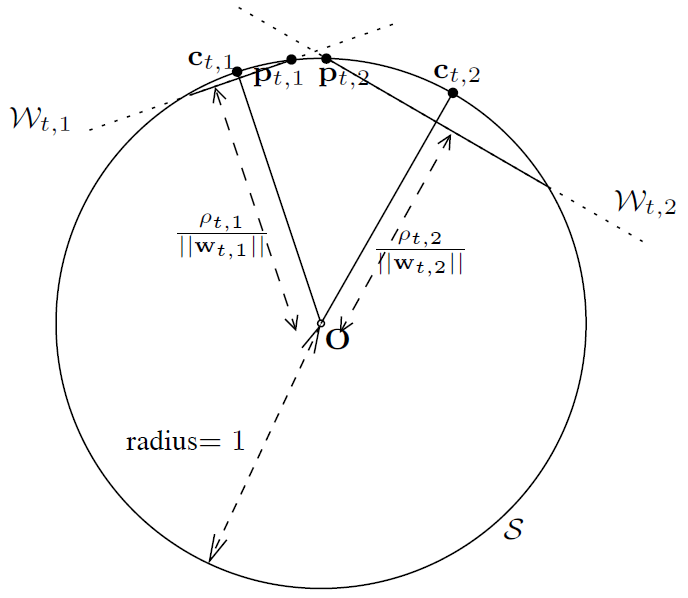
\includegraphics[width=\textwidth]{images/svm}


\begin{itemize}
\item $\alpha_i$ : variables duales
\item $w_i$ : poids de l'hyperplan
\item $\rho_i$ : biais de l'hyperplan
\item $K_{ij}$ : matrice de Gram
\end{itemize}

\end{column}
\end{columns}

\end{frame}

\begin{frame}{Détermination des paramètres $A_i, C$}

\begin{block}{Détermination des paramètres $A_i, C$}
\begin{itemize}
\item Détermination de $A_1$ en essayant différentes valeurs et en visualisant $D$ ($A_2=A_1$).
\item Détermination de $A_2$ en essayant différentes valeurs et en visualisant $D$.
\item Détermination de $C$ visuellement.\\
\textit{Très mauvais résultats avec la méthode de la $p$-valeur avec 200 tirages aléatoires.}
\end{itemize}
\end{block}

\end{frame}

\begin{frame}{Résultat final}{Différence de moyennes}

{
\definecolor{tempGreen}{HTML}{96EAC0}
\setbeamercolor{block body example}{use=structure,fg=black,bg=tempGreen}
\begin{exampleblock}{Distance et ruptures détectées, $A_1 = 20, A_2 = 28, C = 0,6$}
\centering
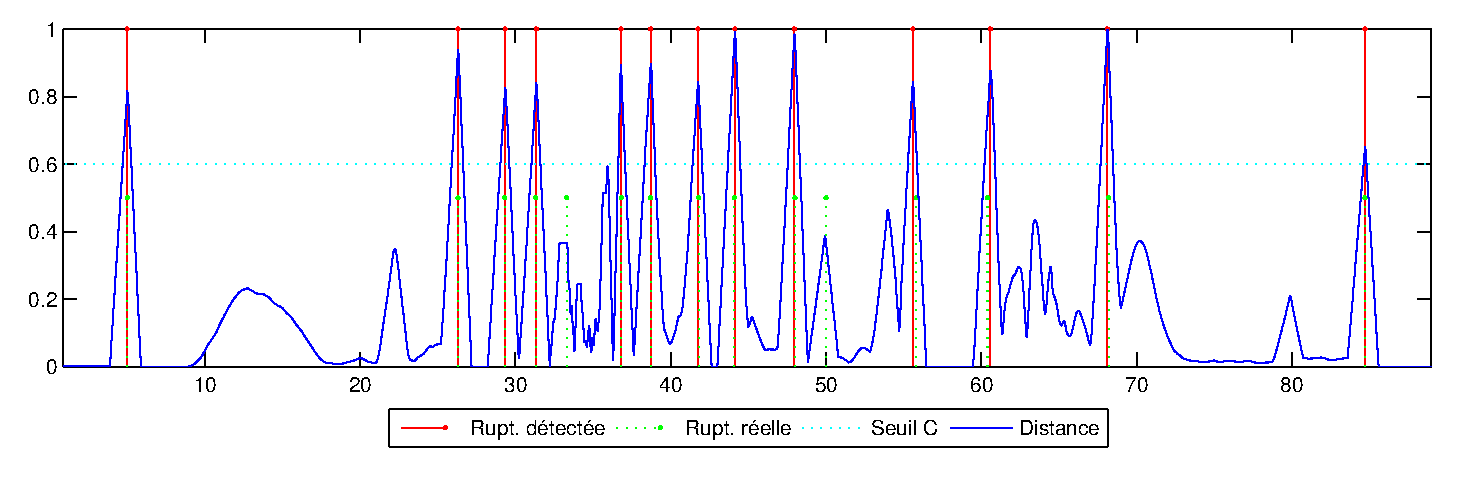
\includegraphics[width=\textwidth]{images/resultatMoy}
\end{exampleblock}
}

\end{frame}

\begin{frame}{Résultat final}{Distance one-class SVM}

{
\definecolor{tempGreen}{HTML}{96EAC0}
\setbeamercolor{block body example}{use=structure,fg=black,bg=tempGreen}
\begin{exampleblock}{Distance et ruptures détectées, $A_1 = 20, A_2 = 28, C = 0,8$}
\centering
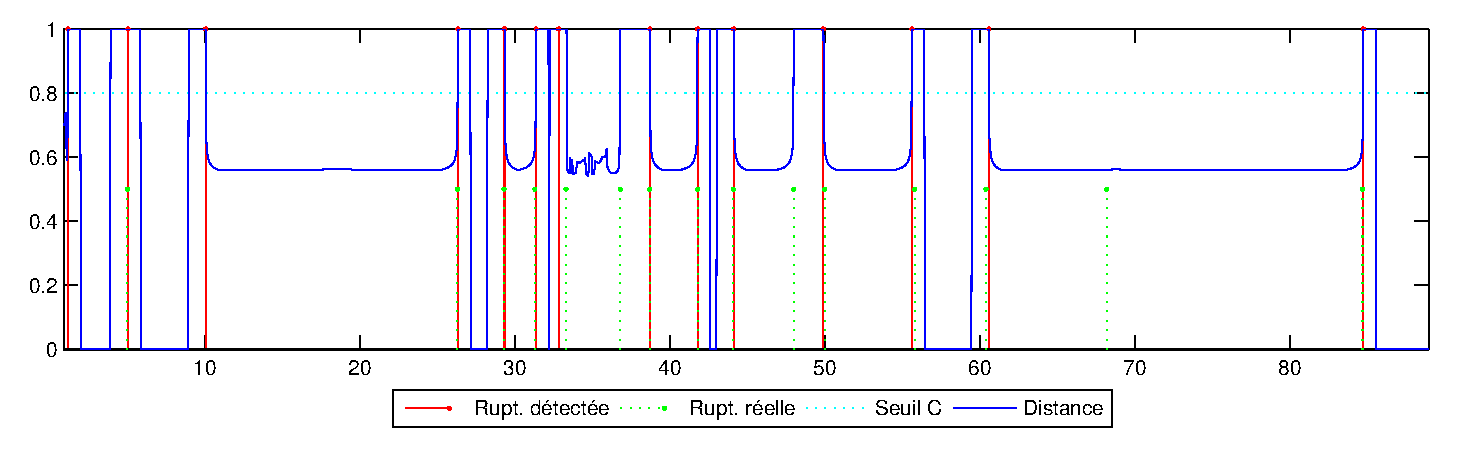
\includegraphics[width=\textwidth]{images/resultatSVM}
\end{exampleblock}
}

\end{frame}


\section{Conclusion}
\subsection{}
\chapter{Conclusion}

Ce projet aura été l'occasion pour nous de réaliser du traitement de vidéo sous forme de détection de rupture.

Nous avons ainsi commencé par la phase classique d'extraction de caractéristiques de la vidéo, une phase que l'on retrouve dans la plupart des problèmes de \textit{Machine Learning} sur des images ou des vidéos, où il est nécessaire d'extraire l'information du signal d'origine pour simplifier et améliorer le processus de traitement et baisser la dimensionnalité du problème \textit{(curse of dimensionality)}.

Ce fut donc pour nous l'occasion d'être confronté à ce problème, qui nous a permis d'extraire des histogrammes RGB et YCbCr, mais également des matrices de coocurrence et le gradient de l'image.

Nous avons également été confronté à la nécessité de prétraiter la matrice de caractéristiques afin de faire ressortir les faibles valeurs et atténuer les fortes valeurs.

Cette phase a été suivie de la détection de rupture utilisant deux types de distance, une distance « simple » qu'est la somme des différence des moyennes, et une distance plus complexe basée sur les paramètres de \textit{SVM one-class}. Les deux ayant fourni des résultats assez bons.

Les axes d'amélioration de notre projet se situent sans doute dans l'essai d'autres caractéristiques qui pourraient peut-être être plus robustes aux variations à l'intérieur d'une scène. Concernant les méthodes de détection de rupture, nous n'avons pas trouvé de méthode alternative importante à celle de la dérivée filtrée. En revanche, il pourrait être intéressant de travailler sur des indicateurs $\hat{\theta}$ et des distances $D$ différentes et qui permettraient une meilleure détection de rupture.


\section{Bibliographie}
\begin{frame}[allowframebreaks]{Bibliographie}
\bibliographystyle{abstract}
\bibliography{../rapport/include/biblio}
 \end{frame}

\end{document}

